%%% Template File for Use with the cmccapstone.cls.

%%%%%%%%%%%%%%%%%%%%%%%%%%%%%%%%%%%%%%%%%%%%%%%%%%%%%%%%%%%%
%%% THE FOLLOWING COPYRIGHT NOTICE SHOULD BE REMOVED FROM FINAL SUBMISSIONS.
%%% THIS IS INCLUDED FOR PUBLIC SHARING

%%% Copyright (C) 2020 Claremont McKenna College

%%% This LaTeX template was originally created for HMC Clinic by
%%% Claire Connelly <cmc@math.hmc.edu>
%%%
%%% Modified by Jeho Park <jeho.park@cmc.edu> to fit the template format to CMC Data Science Capstone Report
%%% Last Modification Date: 5/6/2020

%%% See the COPYING document, which should accompany this
%%% distribution, for information about distribution and modification
%%% of the document and its components.

%%% END COPYRIGHT NOTICE.
%%%%%%%%%%%%%%%%%%%%%%%%%%%%%%%%%%%%%%%%%%%%%%%%%%%%%%%%%%%%

%%%%%%%%%%%%%%%%%%%%%%%%%%%%%%%%%%%%%%%%%%%%%%%%%%%%%%%%%%%%
%%% Note that for *your* final report, you should remove any      
%%% comments that aren't relevant to your report.  
%%% Note that you should also remove the copyright notice assigning 
%%% copyright to the College
%%% Note that depending on your sponsor, you may need to assign  
%%% copyright to the sponsoring organization. Double check with your sponsor. 
%%%%%%%%%%%%%%%%%%%%%%%%%%%%%%%%%%%%%%%%%%%%%%%%%%%%%%%%%%%%

%%% Preamble.

%%% The top part of your document is called the preamble.  You supply
%%% some basic information about the document (such as its title and
%%% author) in a form that LaTeX can understand here.


%%% The first *active line* in your LaTeX document is the \documentclass
%%% command, which loads a LaTeX class file.  Class files generally
%%% define the appearance of a document, and include a variety of
%%% structural commands.

%%% CMC Data Science Capstone reports use the cmccapstone class, which should be located
%%% somewhere in TeX's search path or simple in the same folder/directory with this LaTeX document

%%% You must set a document-class option here (no need to change for your final report)
\documentclass{cmccapstone}

%%% You can load additional LaTeX packages, or style files, that
%%% affect the way that the document is laid out, typeset, or
%%% supply additional commands or environments.  

%%% Keep in mind that the class file already loads many packages
%%% for you; check the documentation or look for the
%%% \RequirePackage lines to see what's loaded.

%%%  !!! If you want to use the amsthm package (AMS theorems
%%%  !!! package), specify "amsthm" in your document-class
%%%  !!! options, which will load amsthm in a way that is
%%%  !!! compatible with the class's font selections.

%%% If you choose to use additional packages, make sure that they
%%% appear *before* the line loading hyperref; hyperref changes
%%% pieces of other packages, so it's important that it be loaded
%%% last.

\usepackage{graphicx}           % More control over graphic inclusion.

%%% !!! Load all other packages before this line !!!

%%% (Optional) Load hyperref as the last package
\usepackage[breaklinks=true, bookmarks, pdfpagemode=UseOutlines, pdfpagelayout=SinglePage, hidelinks]{hyperref}

%%% The preamble can also be used to define your own commands and
%%% environments, set some constants that will be used throughout your
%%% document, and so on.

%%% As you may have guessed, LaTeX's comment character is the percent
%%% sign.  Any line that starts with a % will be ignored.  You can
%%% also use the comment character to add comments to the end of a
%%% line that will be parsed by TeX.

%%% The optional \includeonly command allows you to specify the names
%%% of chapters that you want to typeset.  It is useful for debugging
%%% or for working intensely on one particular part of your document
%%% when you don't want to take the time to retypeset the entire document.


%%% This optional command provides additional context around an error.
%%% It can be helpful when tracking down a problem. 
%\setcounter{errorcontextlines}{1000}


%%% Information about this document.

%%% I find it most useful to put identifying information about a
%%% document near the top of the preamble.  Technically, this
%%% information must precede the \maketitle command, which often
%%% appears immediately after the beginning of the document 
%%% environment.  Placing it near the top of the document makes it
%%% easier to identify the document, and keeps it from getting
%%% mixed up with the content of your document.

%%% So, some questions.

%% What is the name of the company or organization sponsoring your project?
\sponsor{Data R Us, LLC}

%% What is the title of your report?
\title{Making Data Work: A Novel Approach}

%% Who are the authors of the report (your team members)?  (Separate
%% names with \and.)
\author{Student A \and Student B \and Student C \and Student D~(Project Manager)}

%% What is your faculty advisor's name?  (Again, separate names with
%% \and, if necessary.)
\advisor{Jane Doe}

%% Liaison's name or names?
\liaison{Samuel Someone}

%% Did you have an outside consultant help you with this project?  Put
%% their names in the \consultant command.
\consultant{Robert Roe}

%% By not specifying a date with the \date command, the date the
%% document is typeset will be added.

%% If you need to put in a specific date, do so with
%%  \date{May 13, 2004}
%% You probably shouldn't, however.

%%% !!! End of information section !!!


%%% New commands and environments.

%%% You can define your own commands and environments here.  If you
%%% have a lot of material here, you might want to consider splitting
%%% the commands and environments into a separate ``style'' file that
%%% you load with \usepackage.

% \newcommand{\coolcommand}[1]{#1 is cool.} % Lets everyone know that
                                % the person or thing that you provide
                                % as the argument to the command is
                                % cool.

% \newcounter{cms}


%%% Some theorem-like command definitions.

%%% The \newtheorem command comes from the amsthm package.  That
%%% package is *not* automatically loaded by the class file, so if
%%% you choose to use these commands, you'll need to specify the
%%% "amsthm" document-class option.

% \newtheorem{thm}{Theorem}[chapter]
% \newtheorem{lem}{Lemma}[chapter]


%%% If you find that some words in your document are being hyphenated
%%% incorrectly, you can specify the correct hyphenation using the
%%% \hyphenation command.  Note that words are separated by
%%% whitespace, as shown below.

\hyphenation{ap-pen-dix wer-ther-i-an}


%%% !!! The start of the document !!!

%% The document environment is the main environment in any LaTeX
%% document.  It contains other environments, as well as your text.

\begin{document}

%%% The front matter of a large document includes the title page or
%%% pages, tables of contents, lists of figures or tables, and so on,
%%% your abstract, a preface or introduction, and so on.  It's
%%% delineated with the \frontmatter command.

\frontmatter


%%% One of the things that the \frontmatter does is make page
%%% numbers appear as lowercase Roman numerals---i, vi, xii, and so
%%% on.

%%% The first thing in the front matter is your title page.  The title
%%% page is formatted by commands in the document class file, so you
%%% don't need to worry about what it looks like -- just putting the
%%% \maketitle command in your document (and filling in the necessary
%%% information for the identification commands above) is enough.

\maketitle


%%% Abstract

\begin{abstract}
  Your abstract should be a \emph{brief} summary of the contents of
  your report.  Don't go into excruciating detail here---there's
  plenty of room for that later.

  If possible, limit your abstract to a single paragraph, as your
  abstract may be used in promotional materials for the Clinic.
\end{abstract}


%%% Table of Contents, List of Figures, and List of Tables.
%%% 
%%% If you don't have any figures or tables in your report, you
%%% should comment out the appropriate command.  If you don't,
%%% you'll get an extra, mostly blank, page in your typeset report.

\tableofcontents
\listoffigures
\listoftables


%%% Acknowledgments.
%%%
%%% This section is to thank individuals or organizations who made contributions to your project.
%%% In addition, you can specify contributions and impacts in detail where appropriate in the body.
%%% 

\begin{acknowledgments}
Thank some people and organizations here, if you like.
\end{acknowledgments}


%%% End of the front matter.
%%%%%%%%%%%%%%%%%%%%%%%%%%%%%%%%%%%%%%%%%%%
%%%%%%%%%%%%%%%%%%%%%%%%%%%%%%%%%%%%%%%%%%%
%%% Beginning of the main matter.

%% The main part of your report consists of normal, numbered
%% chapters as well as any appendices.  Bibliographies, indexes, and
%% so on are part of the back matter.  The main matter is opened with the
%% \mainmatter command.

\mainmatter


%%% Content.

%%% For smaller documents---especially those you're writing by
%%% yourself---you might write your entire report using a single LaTeX
%%% source file.  For larger documents, we recommend that you split
%%% the source file into several separate, smaller files.  The smaller
%%% files are ``included'' into your main, or ``master'' document
%%% using \include commands.

%%% Splitting your source has several advantages.  First, if you're
%%% working on a document with a group of people, it allows you to
%%% have more than one person working on different parts of the
%%% document at the same time (although we still recommend that you
%%% use GitHub, Overleaf, or a similar revision-control system!). 
%%% Second, smaller document chunks allow you to reorganize your 
%%% document more easily.  If you later decide that Chapter 8 would be better as
%%% Chapter 4, all you have to do is swap the \include commands
%%% around.  For that reason, you should give your separate chapters
%%% meaningful names, such as "introduction'', "background'', or
%%% "conclusions'' rather than calling them "chapter1'',
%%% "chapter2'', and so on.

%%% Finally, splitting the document allows you to concentrate on a
%%% particular section without being distracted by other
%%% sections---all you have to do is comment out the \include line for
%%% the sections you're not working on.  This technique can be
%%% especially useful when you're trying to track down a problem by
%%% allowing you to easily locate the file with the problem by
%%% ruling out the other sections.

%%% In our example document, we define several chapters that have
%%% useful information about writing capstone or thesis reports
%%% using LaTeX.  Here, we'll just use placeholders (but not
%%% chapter1, chapter2, etc!).  .


%%% Chapter 1

\chapter{Introduction}\label{Ch:Introduction}

The introduction should describe what the purpose of the project is/was and what you have accomplished.
The introduction, as well as other parts of the report, can be developed incrementally and will evolve with the project.
The introduction should contain the following items:
\begin{enumerate}
\item a brief description of the sponsoring organization (which often can be derived from the organization's online boilerplate), 
\item a suitably condensed statement of the problem posed by the sponsor, 
\item some discussion of the relevance of the project to the sponsor's business, 
\item the team's approach to the problem, gleaned from the team's Statement of Work (including a summary of background study, i.e., literature review, to explain how your work differs from or builds on previous efforts --- this explanation should be reinforced by entries with annotation in the bibliography),
\item summary of the report: in separate paragraphs specify and summarize the major sections of your report (Ch 2, Ch 3, ... , Conclusion,  Appendixes, Glossary, Bibliography).
\end{enumerate}

\begin{quote}
    \S{} \LaTeX{} Tip: When you create your report, we recommend you to create different TeX file for different chapter. In this example, you will also find several LaTeX files comprising multiple chapters as the main body.  
\end{quote}



\endinput % see the "introduction.tex" file

%%% Chapter 2

\chapter{Another Chapter}\label{Ch:another_chapter}

This is another chapter and now you should know how to add more chapters.

The basic structure of the report consists of front matter, main matter, and back matter. 

Front matter includes a Cover Page, an Abstract, Acknowledgments, a Table of Contents, a List of Figures, a List of Tables.

The main matter of the report consists of several chapters, including an Introduction, additional Chapters, and Conclusion.

Back matter may include appendixes, a glossary, a list of abbreviations and Bibliography.

The current version (v.1) includes samples of front matter and main matter. The back matter of this version will be added later for your convenience. 

\endinput

%%% Chapter 3

\chapter{Technical Writing Tips}\label{Ch:technical_writing_tips}

\begin{enumerate}{}
\item Always remember who your audience is. Your readers include both your liason with technical knowledge of you methods to the company executives with a college level, general education knowledge of science.  
\item Always write with pedagogy in mind. You are trying to teach your reader what is it you did, what the techniques are based off of, and what they can be used for.  
\item Don't fall into the trap of trying to sound smart and display what you know. If you're using technical jargon unnecessarily, you will only confuse and frustrate your audience. 
\item Technical writing is succinct and to the point. Each sentence needs to be short, often single clauses and use accessible, non-flowery language. 
\item Avoid run-on sentences. The words "which" and "where" are your enemy here because they are often used to combine clauses and increase the word length of your sentences. Of course, having shorter sentences might increase the length of your document, but reading a lot of simple, readable text is far better than slowly slogging through dense, erudite text.
\item Avoid repetition. You might need to repeatedly refer to some important word in your document (think "data," or "system," or "model"). But if the reader keeps reading the same word over and over again in adjacent sentences, it starts to ring in their head and the writing comes off amateurish. Reword to avoid repetition.
\item Citations, citations, citations; do not forget to cite relevant work or facts you mention. The rule of thumb is that if you say a fact that is both non-obvious and for which you personally did not perform the experiment to demonstrate, then you must cite something.
\item The usual English writing rules still hold: avoid ending your sentences in prepositions; avoid passive voice; don't start sentences with numerals; etc.
\end{enumerate}


\endinput

%%% Chapter 4

\chapter{Creating Figures}\label{Ch:creating_figures}

Example text preceding the figure command.
%
\begin{figure}%[optional modifiers]
    \centering
    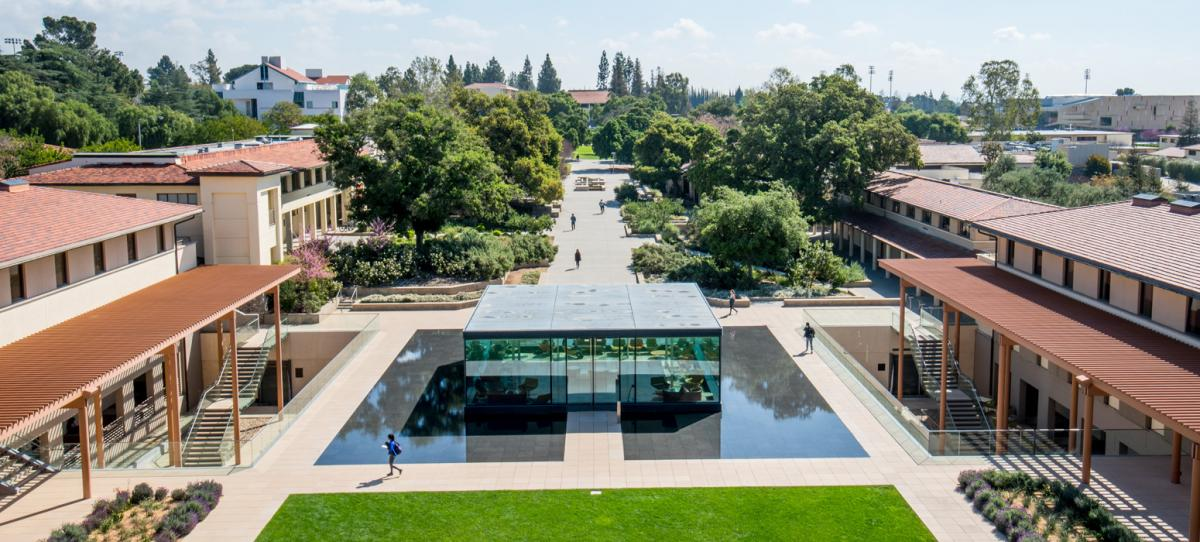
\includegraphics[width=5cm]{Graphic1.jpg}
    \qquad %For a sufficient space between side by side graphics
    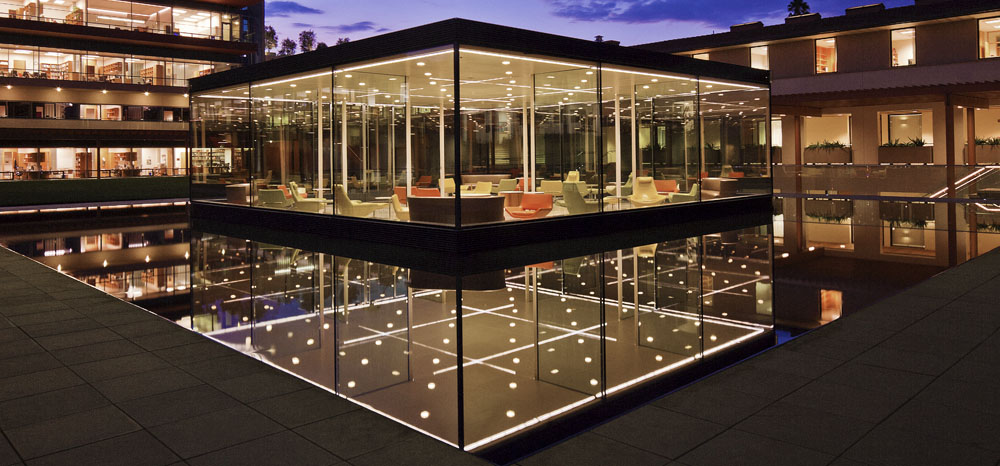
\includegraphics[width=5cm]{Graphic2.jpg}
    \caption{Very short gist of the point of this figure's inclusion. (a) Long, descriptive caption of the first graphic. (b) Long, descriptive caption of the second graphic.}
    \label{FIG_DESCRIPTIVELABEL}
\end{figure}
%
Example text post the figure command; still part of the same paragraph.

Example text for the following paragraph. Note that Latex places the figure close to where you called the command, but not exactly there. 

\begin{enumerate}
    \item Modifiers right after the begin command can change the figure location (ex. [t] can force the location at the top of a page).
    \item Make your captions descriptive enough so that someone who reads nothing else in your paper can still get the gist of the idea.
    \item EVERY figure needs to be referenced in the document and in the order in which they are presented.
    \item Plots must not depend on colors to differentiate between graphs. Alternative methods include dotted or dashed lines or identifying token at graph vertices. Using color is, of course, still welcome, but must be a supplement.
    \item All axis of a plot must be labeled with nicely readable and large fonts.
    \item If there are more than two graphics in a figure, they must each be labeled (as part of the graphic) with a letter (a), (b), (c), etc. Each graphic must be described in the caption.
\end{enumerate}





\endinput

%%% Chapter 5

\chapter{Equation Etiquette}\label{Ch:equation_etiquette}

This is an example of an equation that comes at the end of a sentence:
%
\begin{equation}
    \mathrm{Area} = \pi r^2.
\end{equation}
%
Note the above has a period at the end of the equation because it was at the end, but the following equation,
%
\begin{equation}
    p_{\mathrm{Normal}}(x\vert \mu, \sigma^2) = \frac{1}{\sqrt{2 \pi \sigma^2}}\mathrm{exp}\left[-\frac{(x - \mu)^2}{2 \sigma^2}\right],
\end{equation}
%
has a comma at the end because it's in the middle of a sentence.

Here's an example of a multi line equation using the align command:
%
\begin{align}
    \mathrm{E}[X] &= \sum_{n=1}^{6} n \mathrm{Pr}(X=n)\nonumber\\
    &= \sum_{n=1}^{6} n \frac{1}{6}\nonumber\\
    &= 3.6.
\end{align}
%
Take note of the use of the nonumber command to suppress the extra equation numbers.


\begin{enumerate}{}
\item Use equation for single line equations and use align for multiple line equations.
\item For multiple line equations, use nonumber to suppress the extra equation numbers.
\item Math symbols and variables are italicized; English words are not. Thus, use mathrm when in Mathmode to specify the English words. This is a subtle point, but subscripts and function names that are actually abbreviations of English words should still be treated as normal English.
\item Surround your equation/align commands by \% so that there are no unintentional new paragraphs while making your Latex more readable.
\item Math equations are part of your sentence, so use punctuation accordingly: if the equation is at the end, use a period; if the equation is in the middle of your sentence, use a comma.
\item Create labels for your equations and when you reference them, use the tilda to create a small space as so: You can find the result in Eq.\textasciitilde\textbackslash ref\{EQ\_IMPORTANTRESULT\}.
\item For inline math, surround your math with dollar signs. Keep in mind the format might look a little different to fit large symbols, such as in $\sum_{n=1}^{6} \frac{1}{6} = 1$.
\end{enumerate}


\endinput

%%% Chapter 6

\chapter{Formatting your Bibliography}\label{Ch:formatting_your_bibliography}

Create a separate .bib file and fill it with bib entries for each paper or book you read as follows:\\

%% The following is an example entry to display in the body
%% Look at the our_bib_file.bib for the correct format
\noindent @article\{Gerdil2003,\\
	Author = \{Catherine Gerdil\},\\
	Title = \{\{The Annual Production Cycle for Influenza Vaccine\}\},\\
	Journal = \{Vaccine\},\\
	Volume = \{21\},\\
	Pages = \{1776--1779\},\\
	Year = \{2003\}\\
	\}


\begin{enumerate}{}
\item Use double curly brackets around the title to force formatting that way you type it. Otherwise, depending on the bibliography style set, Latex might auto sentence-case your title and made abbreviations not show up in all caps. 
\item Use two minus signs for a dash between page numbers.
\item Only sources that are cited in your document with the cite command will show up in your bibliography, typically in the order in which you cite them (dependent on bibliography style).
\item If you are citing a fact, you cite at the end of the sentence that first mentions that fact. There is no need to recite in the document for the same fact.
\item If you are mentioning explicitly a paper, book, or other citable document, you cite immediately after that mention. Keep in mind there needs to be a space between the cite command and the last word. 
\item When citing a source with multiple authors, you refer to it as "first\_author's\_last\_name et al." and then immediately cite.
\item Citations appear before the period that ends the sentence. 
\item BE CAREFUL of the export citation tools found on journal websites. What often comes out is riddled with errors. If you choose to use them (I suggest you don't and just type everything out yourself), go through with a fine comb and check your bibliography for errors. 
\end{enumerate}


\endinput


%%% Appendices.

%%% Appendices are just like chapters, only they're generally
%%% lettered rather than numbered (although that depends on your
%%% document class, of course).

%%% The appendices are delineated with the \appendix command.
%%% Individual appendices are begun with the standard \chapter or
%%% \section commands.  In our example, we'll \include them just as
%%% we did other chapters.

%%% If you don't have any appendices, comment out the \appendix
%%% command.

\appendix

\include{our_appendix}

\include{our_source_code}

%%% End of the main matter.
%%%%%%%%%%%%%%%%%%%%%%%%%%%%%%%%%%%%%%%%%%%
%%%%%%%%%%%%%%%%%%%%%%%%%%%%%%%%%%%%%%%%%%%
%%% Beginning of the back matter.

%%% The back matter of a document is where the bibliography, index,
%%% glossary, and other unnumbered chapters or sections occur.  It
%%% starts, not surprisingly, with the \backmatter command.

\backmatter


%%% Bibliography.

%%% BibTeX is the tool to use for citations and layout of your
%%% bibliography.  Instead of having to type ``[5]'' or ``(Jones,
%%% 1968)'' (and keep track of which citation is which and renumber
%%% them as you add more references to your bibliography), you use
%%% special commands that allow BibTeX and LaTeX to automatically put
%%% the correct information in the right place.

%%% Depending on your field, it may or may not be appropriate to list
%%% references for which you haven't included specific citations.  If
%%% your field sanctions such practices, or if you just want to get an
%%% idea of what you have in your bibliography file, you can include
%%% everything with the \nocite{*} command.
\nocite{*} 


%%% The appearance of your bibliography and citations in your text are
%%% defined by a combination of any bibliography-related LaTeX
%%% packages (such as natbib, harvard, or chicago) and the particular
%%% bibliography style file that you load with the \bibliographystyle
%%% command.  
%%% Note that bibliography-style files have .bst file extension.

% Standard bibliography style.
% Here we use HMC math bibliography-style file as an example.
\bibliographystyle{hmcmath}

% Annotated bibliography style.
% \bibliographystyle{hmcmathannote}


%%% The particular bibliography data file or files that you want to
%%% use are specified with the \bibliography file.  Multiple files are
%%% separated by commas.

%%% You might want to use multiple bibliography (or "bib'') files if
%%% you had a master bib file containing references you use again and
%%% again, and another containing only records for references for a
%%% particular project.

%%% Many people create a single, large bib file that they use for
%%% everything they write.  That approach requires you to \cite every
%%% reference that you want to use in your document -- using
%%% \nocite{*} with a huge bibliography database will give you a large
%%% bibliography containing many references you haven't consulted for
%%% your particular document!

\bibliography{our_bib_file}


%%% Glossary or Index.

%%% If you were going to include a glossary or index in your document,
%%% the relevant commands would appear here.

%%% If you think that you would like to include such features, talk
%%% with someone who's worked with LaTeX a lot very early in your
%%% writing process.  These commands require you to do a bit of
%%% thinking about what you would want to index or gloss in
%%% advance---going back though a completed document to add \index
%%% commands is *not fun*.


\end{document}



%%% Local Variables:
%%% mode: latex
%%% TeX-master: t
%%% End:
